\chapter{DMC}

Zaimplementowałem pięć regulatorów, tj. analityczny, numeryczny, z sukcesywną linearyzacją, nieliniową predykcją i linearyzacją oraz regulator rozmyty. Pominąłem regulator z nieliniową optymalizacją, ze względu trudność jego praktycznego zastosowania - niemożliwy do oszacowania czas znalezienia minimum. Wygenerowano sekwencję sygnału zadanego, taką samą dla każdego z regulatorów. W każdym z regulatorów uwzględniłem pomiar zakłócenia.

\begin{lstlisting}[style=Matlab-editor]
%% DMC(N, Nu, D, D_disturbance, lambda)
dmc = DMC(100, 2, 150, 150, 1);
% Pierwsza iteracja jest wspólna dla wszystkich algorytmów DMC
dmc.dynamic_matrix(s);
dmc.past_matrix(s);
dmc.matrix_disturbance(s_disturbance);

% Test
y_zad = [repelem((rand(1, obiekt.kk/250) * 40 - 20), 250)];
y_zad(1:100) = 0;
u_D = [repelem((rand(1, obiekt.kk/200) * 10 - 5), 200)];

pool = gcp();
f.analiticHammerstein = parfeval(pool, ...); 
f.analiticWiener = parfeval(pool, ...);
f.numericHammerstein = parfeval(pool, ...);
f.numericWiener = parfeval(pool, ...);
f.slHammerstein = parfeval(pool, ...); 
f.slWiener = parfeval(pool, ...);
f.nplHammerstein = parfeval(pool, ...);
f.nplWiener = parfeval(pool, ...);
f.fuzzyHammerstein = parfeval(pool, ...);
f.fuzzyWiener = parfeval(pool, ...);

fprintf("\nFunkcje uruchomione asynchronicznie...\n\n");
\end{lstlisting}

\newpage
\newgeometry{left=1mm, right=1mm, top=25mm, bottom=25mm} 

\begin{figure}[b!]
\centering
\begin{subfigure}[b]{0.49\paperwidth}
\centering
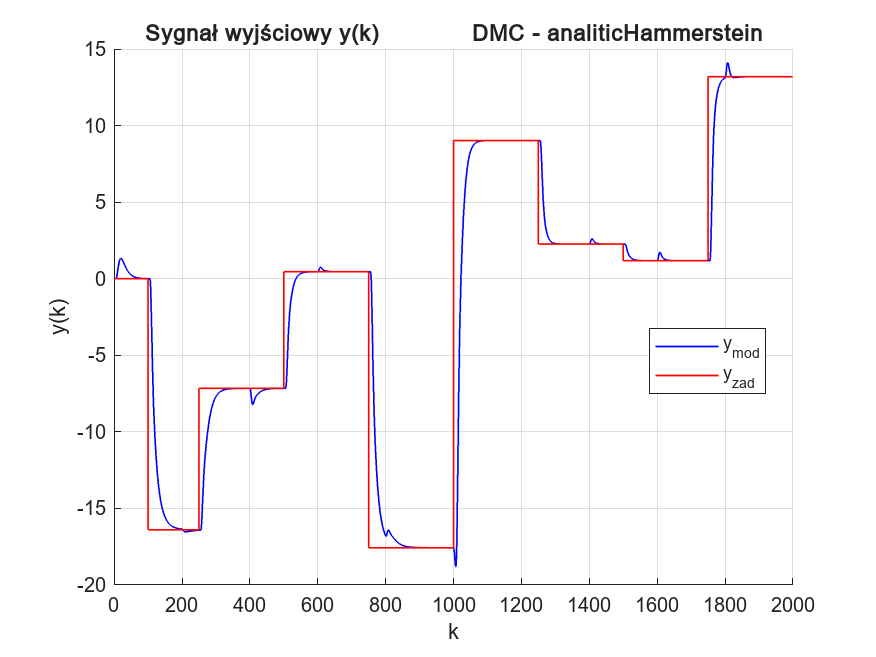
\includegraphics[width=\linewidth]{pictures/y_analiticHammerstein}
\caption{Hammerstein - sygnał wyjściowy $y(k)$.}
\end{subfigure}
\hfill
\begin{subfigure}[b]{0.49\paperwidth}
\centering
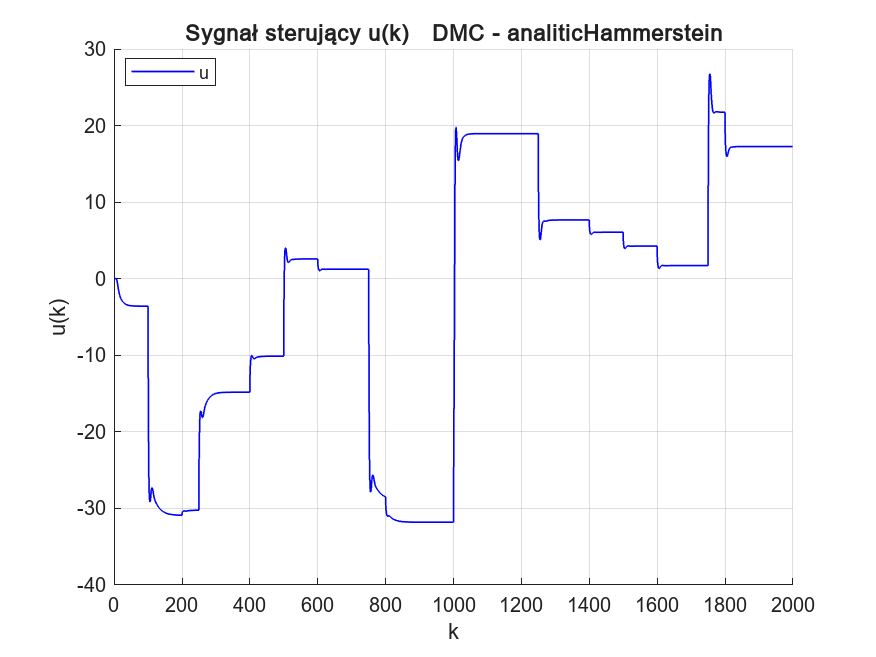
\includegraphics[width=\linewidth]{pictures/u_analiticHammerstein}
\caption{Hammerstein -  sygnał sterujący $u(k)$.}
\end{subfigure}
    
\vspace{0.5cm} % Dystans pionowy między rzędami

\begin{subfigure}[b]{0.49\paperwidth}
\centering
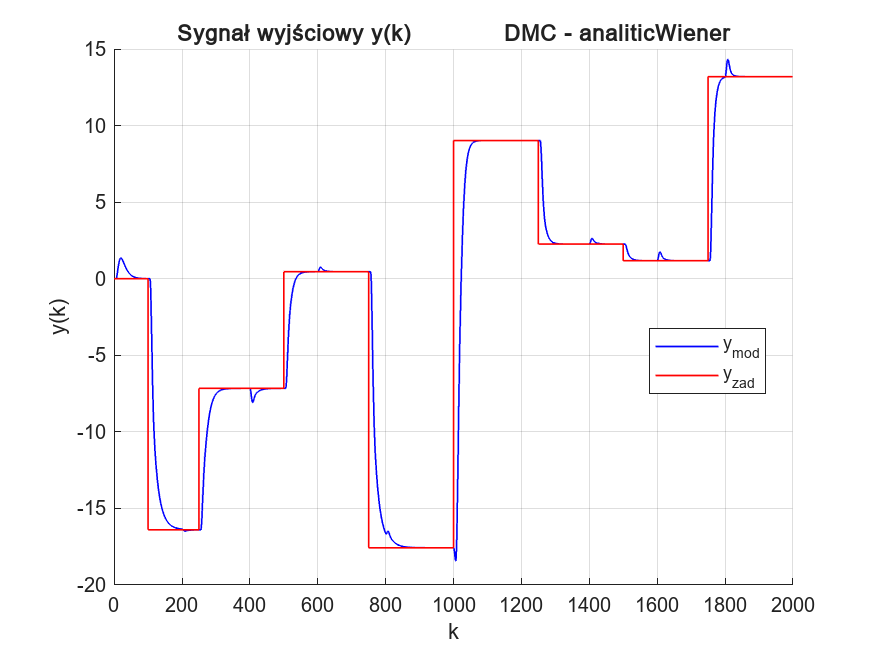
\includegraphics[width=\linewidth]{pictures/y_analiticWiener}
\caption{Wiener - sygnał wyjściowy $y(k)$.}
\end{subfigure}
\hfill
\begin{subfigure}[b]{0.49\paperwidth}
\centering
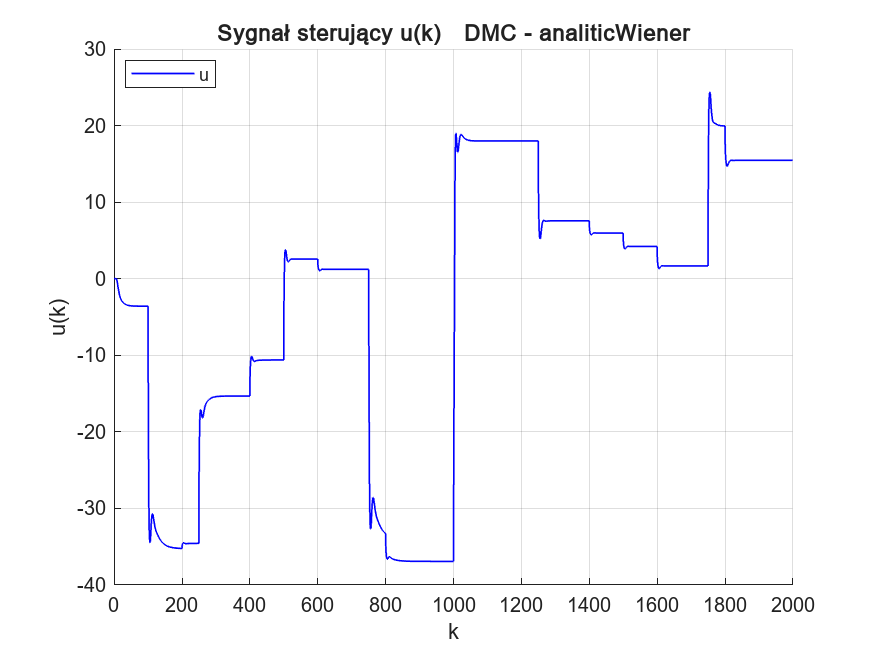
\includegraphics[width=\linewidth]{pictures/u_analiticWiener}
\caption{Wiener - sygnał sterujący $u(k)$.}
\end{subfigure}

\caption{Regulator analityczny.}
\end{figure}

\newpage

\begin{figure}[b!]
\centering
\begin{subfigure}[b]{0.49\paperwidth}
\centering
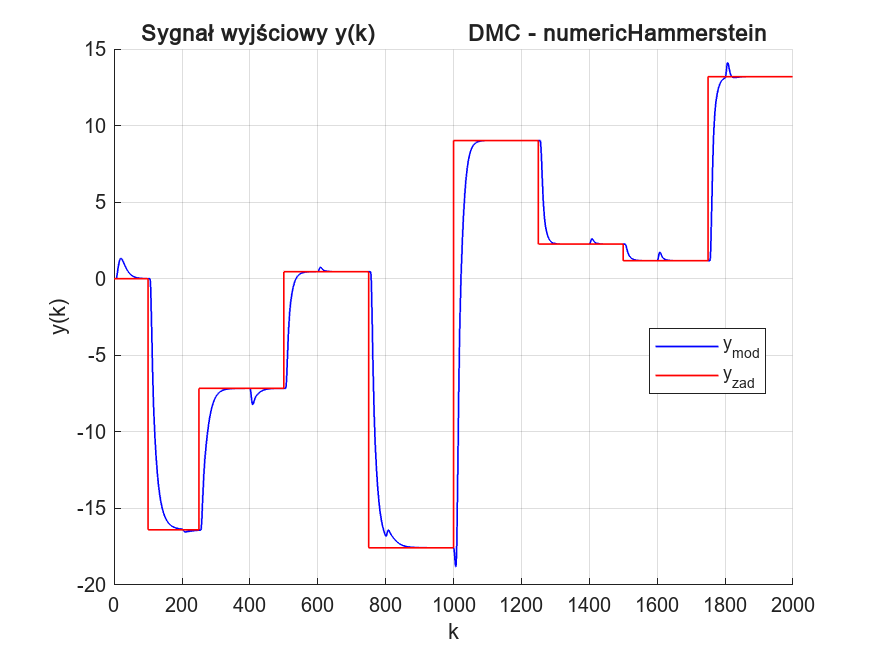
\includegraphics[width=\linewidth]{pictures/y_numericHammerstein}
\caption{Hammerstein - sygnał wyjściowy $y(k)$.}
\end{subfigure}
\hfill
\begin{subfigure}[b]{0.49\paperwidth}
\centering
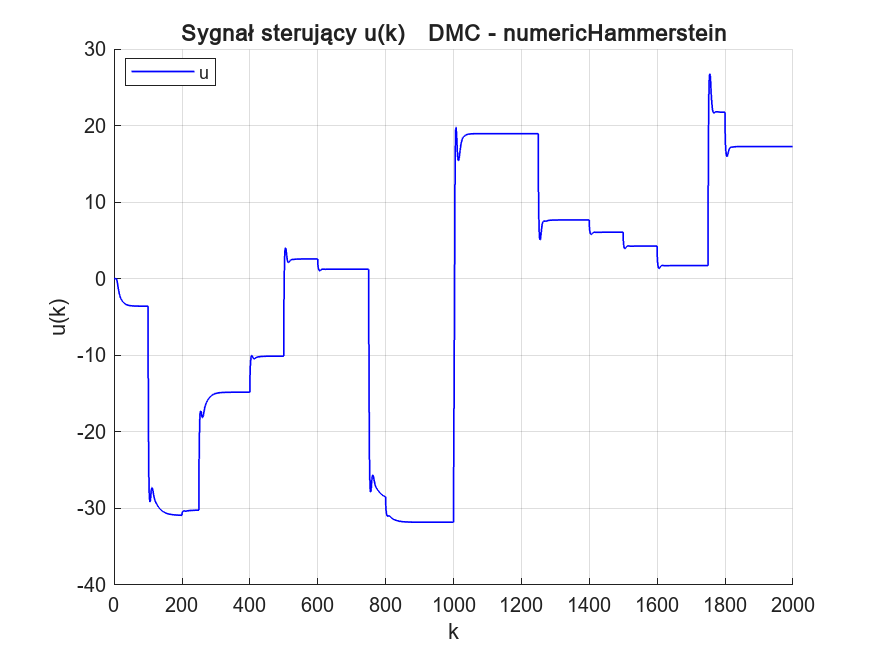
\includegraphics[width=\linewidth]{pictures/u_numericHammerstein}
\caption{Hammerstein -  sygnał sterujący $u(k)$.}
\end{subfigure}
    
\vspace{0.5cm} % Dystans pionowy między rzędami

\begin{subfigure}[b]{0.49\paperwidth}
\centering
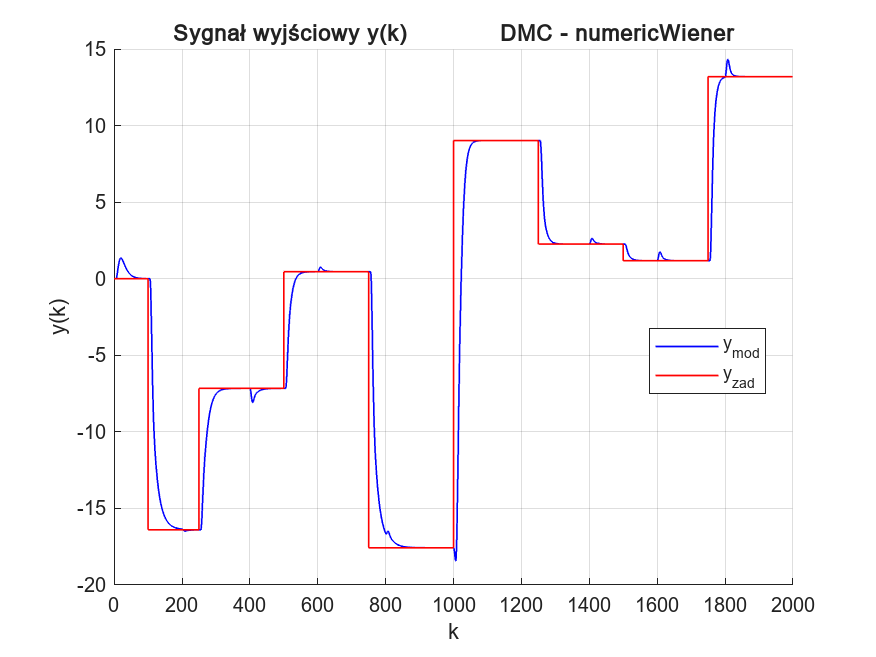
\includegraphics[width=\linewidth]{pictures/y_numericWiener}
\caption{Wiener - sygnał wyjściowy $y(k)$.}
\end{subfigure}
\hfill
\begin{subfigure}[b]{0.49\paperwidth}
\centering
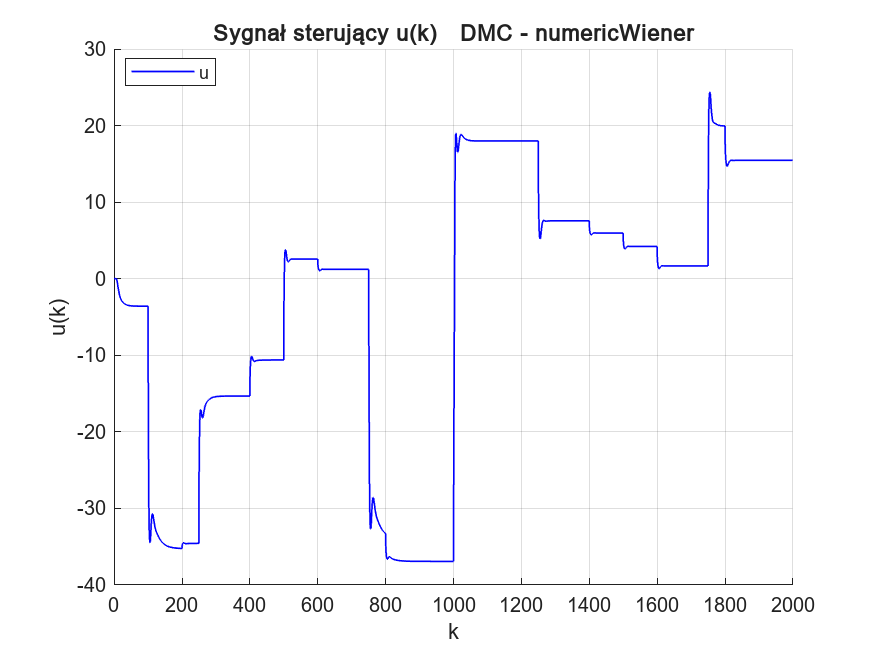
\includegraphics[width=\linewidth]{pictures/u_numericWiener}
\caption{Wiener - sygnał sterujący $u(k)$.}
\end{subfigure}

\caption{Regulator numeryczny.}
\end{figure}

\newpage

\begin{figure}[b!]
\centering
\begin{subfigure}[b]{0.49\paperwidth}
\centering
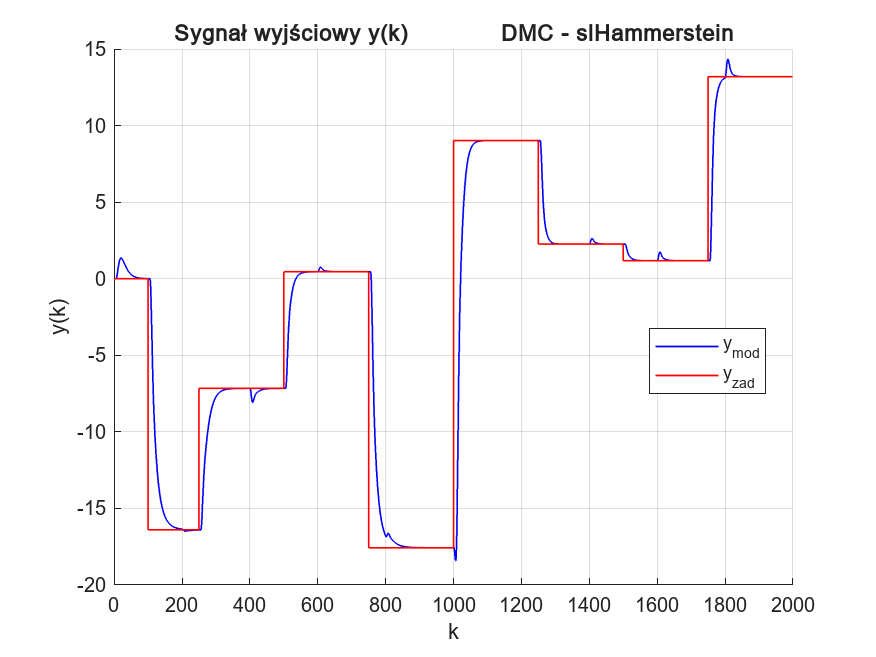
\includegraphics[width=\linewidth]{pictures/y_slHammerstein}
\caption{Hammerstein - sygnał wyjściowy $y(k)$.}
\end{subfigure}
\hfill
\begin{subfigure}[b]{0.49\paperwidth}
\centering
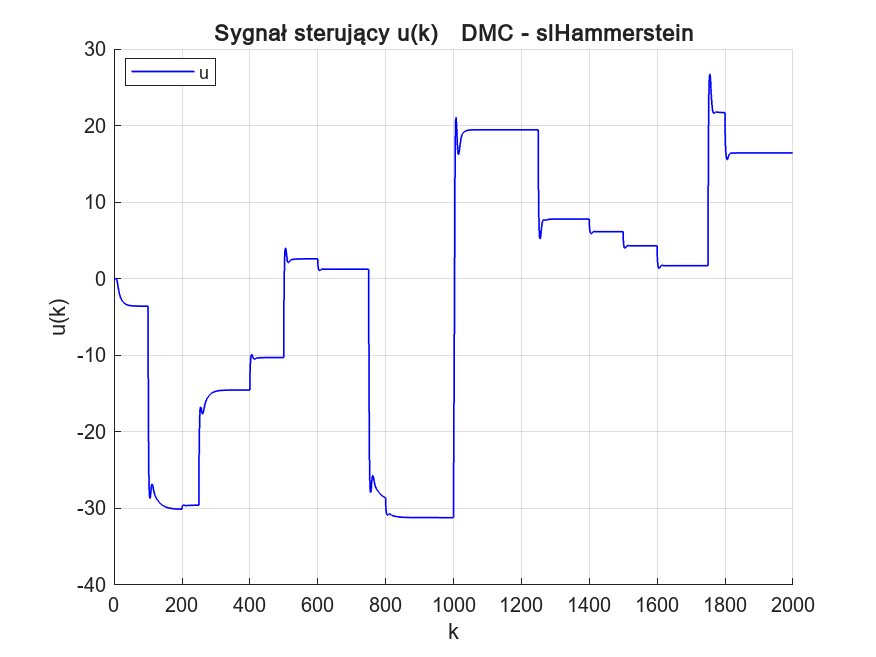
\includegraphics[width=\linewidth]{pictures/u_slHammerstein}
\caption{Hammerstein -  sygnał sterujący $u(k)$.}
\end{subfigure}
    
\vspace{0.5cm} % Dystans pionowy między rzędami

\begin{subfigure}[b]{0.49\paperwidth}
\centering
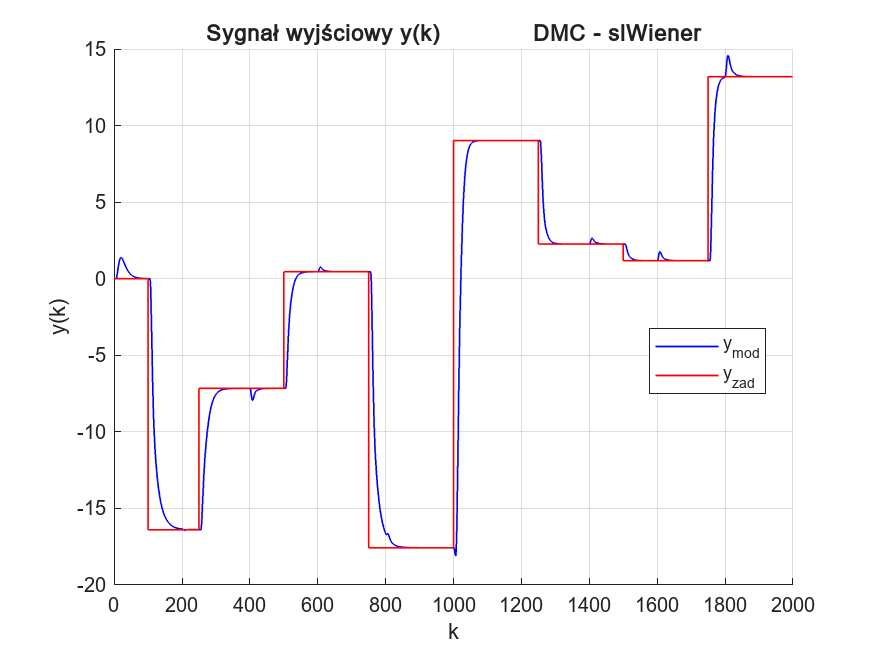
\includegraphics[width=\linewidth]{pictures/y_slWiener}
\caption{Wiener - sygnał wyjściowy $y(k)$.}
\end{subfigure}
\hfill
\begin{subfigure}[b]{0.49\paperwidth}
\centering
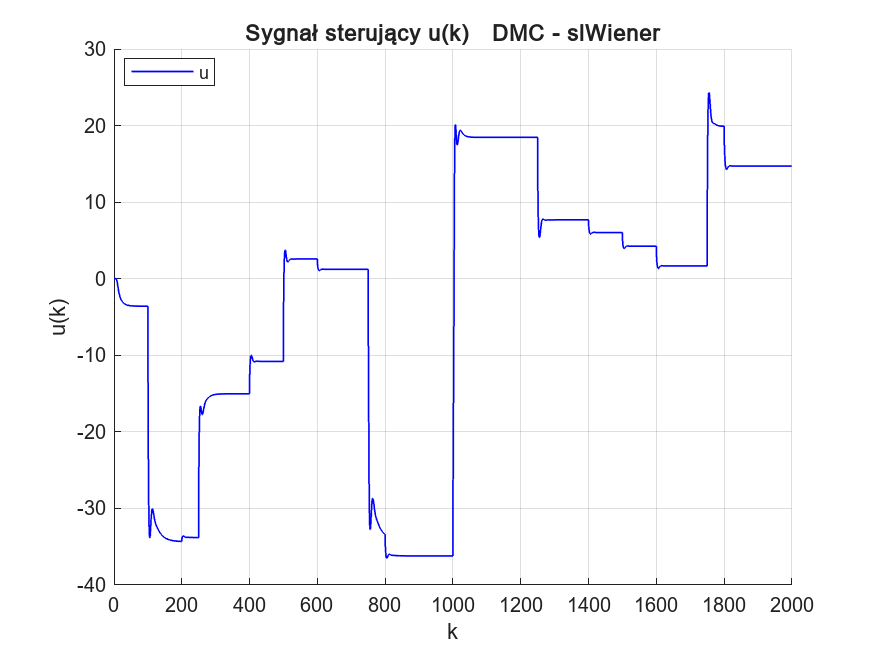
\includegraphics[width=\linewidth]{pictures/u_slWiener}
\caption{Wiener - sygnał sterujący $u(k)$.}
\end{subfigure}

\caption{Regulator DMC-SL.}
\end{figure}

\newpage

\begin{figure}[b!]
\centering
\begin{subfigure}[b]{0.49\paperwidth}
\centering
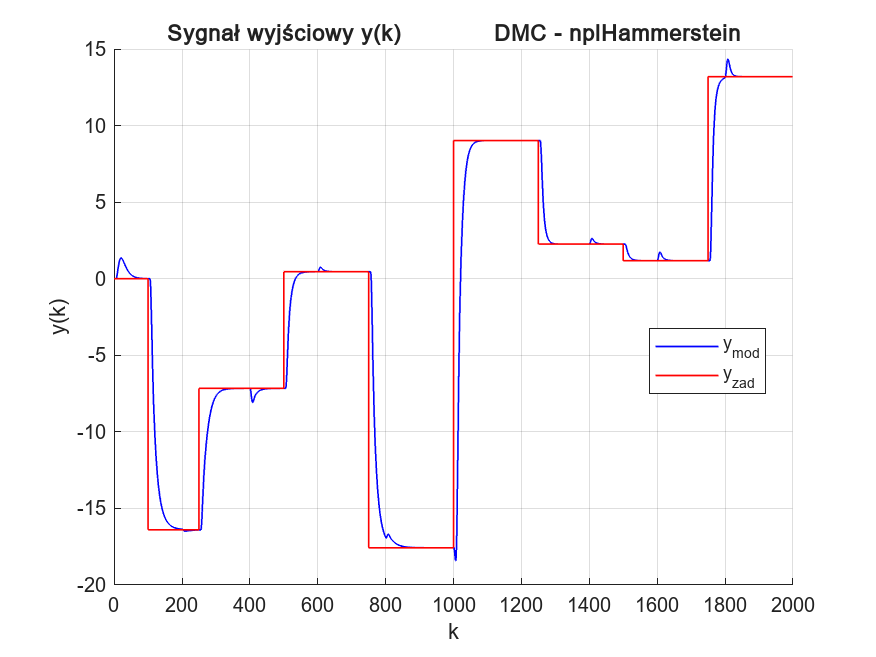
\includegraphics[width=\linewidth]{pictures/y_nplHammerstein}
\caption{Hammerstein - sygnał wyjściowy $y(k)$.}
\end{subfigure}
\hfill
\begin{subfigure}[b]{0.49\paperwidth}
\centering
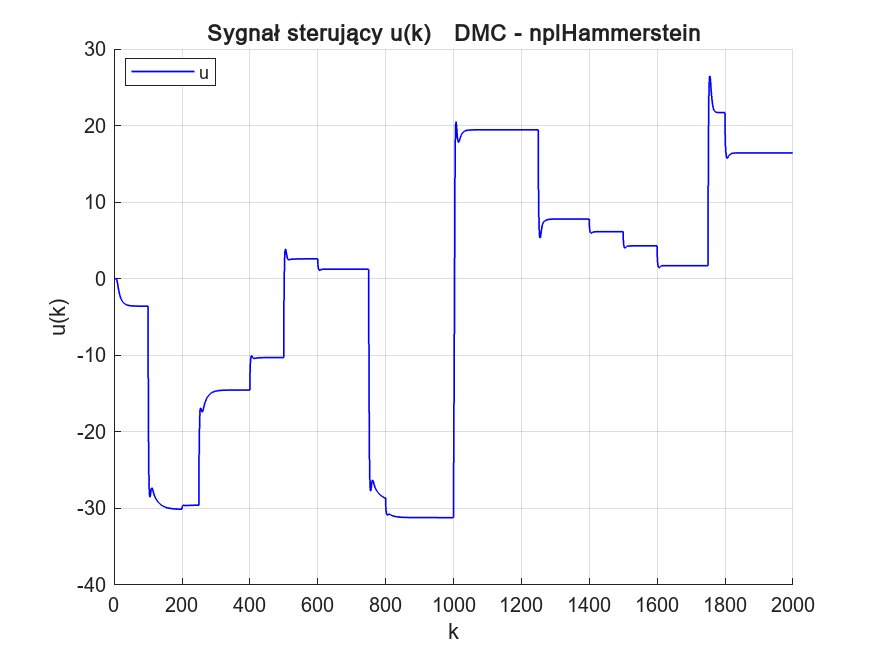
\includegraphics[width=\linewidth]{pictures/u_nplHammerstein}
\caption{Hammerstein -  sygnał sterujący $u(k)$.}
\end{subfigure}
    
\vspace{0.5cm} % Dystans pionowy między rzędami

\begin{subfigure}[b]{0.49\paperwidth}
\centering
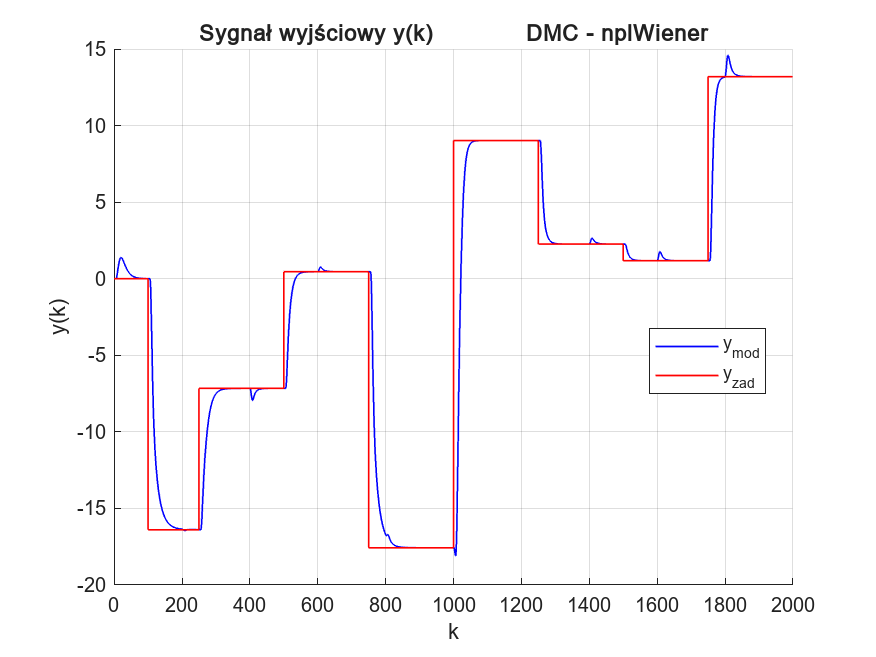
\includegraphics[width=\linewidth]{pictures/y_nplWiener}
\caption{Wiener - sygnał wyjściowy $y(k)$.}
\end{subfigure}
\hfill
\begin{subfigure}[b]{0.49\paperwidth}
\centering
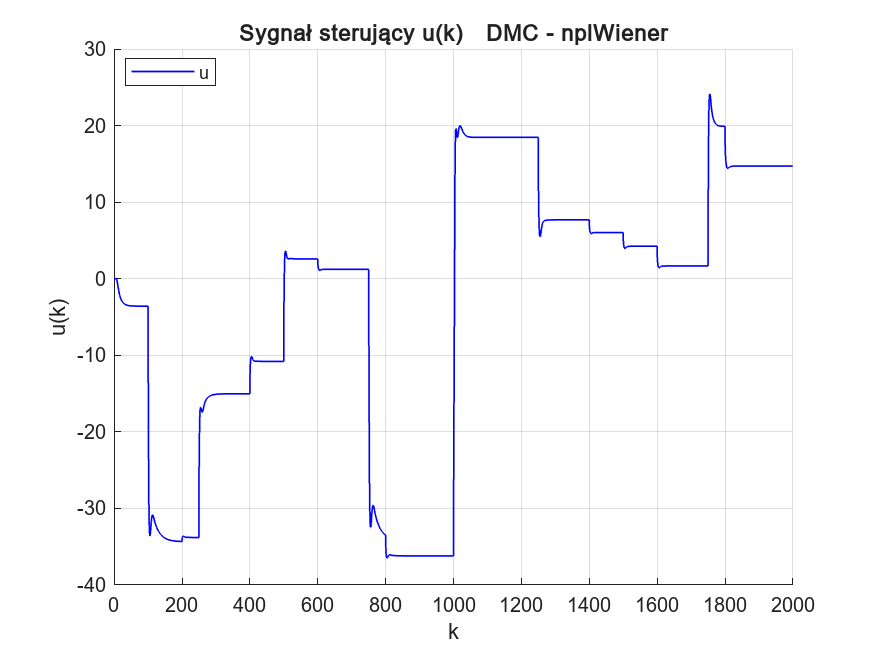
\includegraphics[width=\linewidth]{pictures/u_nplWiener}
\caption{Wiener - sygnał sterujący $u(k)$.}
\end{subfigure}

\caption{Regulator DMC-NPL.}
\end{figure}

\newpage

\begin{figure}[b!]
\centering
\begin{subfigure}[b]{0.49\paperwidth}
\centering
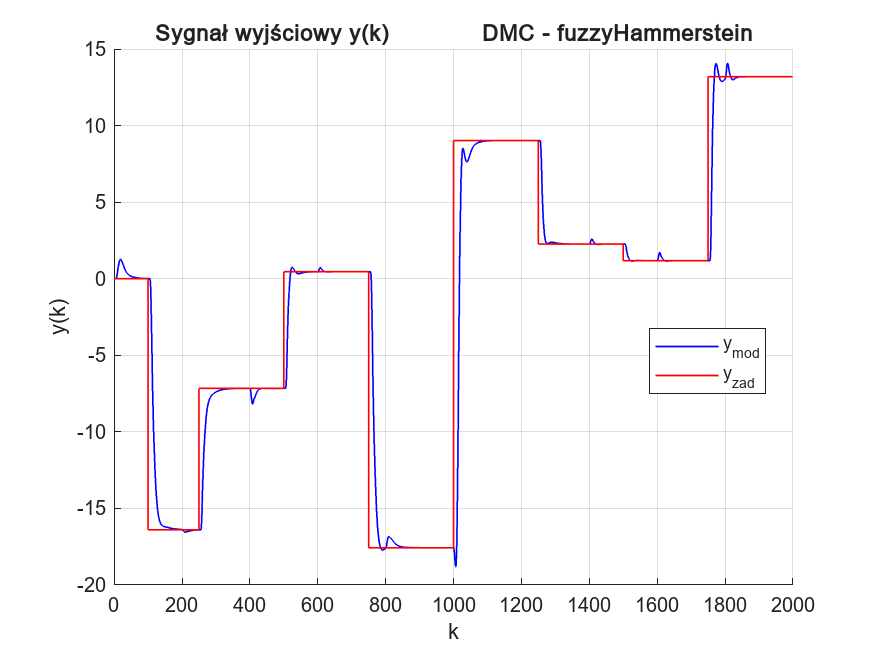
\includegraphics[width=\linewidth]{pictures/y_fuzzyHammerstein}
\caption{Hammerstein - sygnał wyjściowy $y(k)$.}
\end{subfigure}
\hfill
\begin{subfigure}[b]{0.49\paperwidth}
\centering
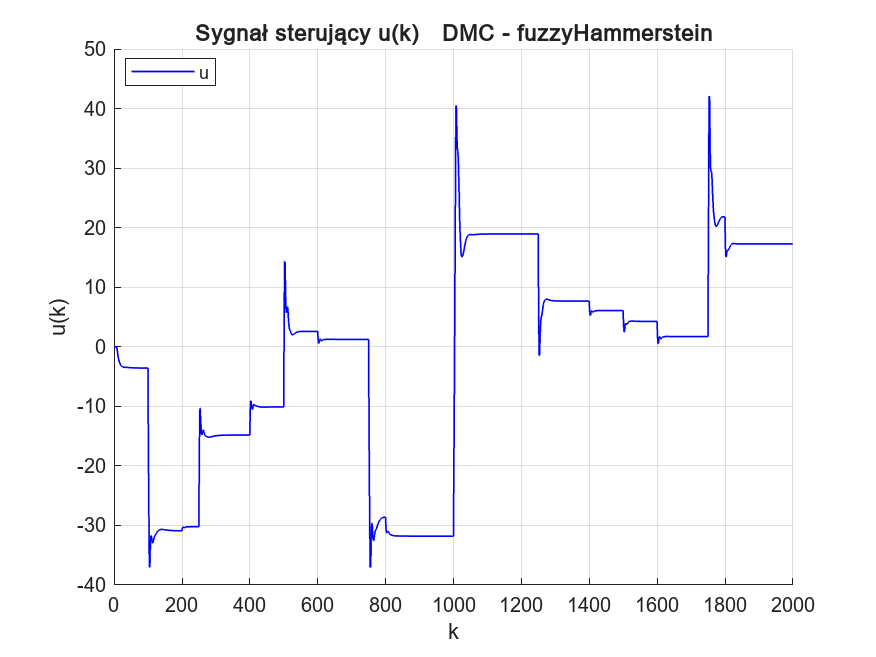
\includegraphics[width=\linewidth]{pictures/u_fuzzyHammerstein}
\caption{Hammerstein -  sygnał sterujący $u(k)$.}
\end{subfigure}
    
\vspace{0.5cm} % Dystans pionowy między rzędami

\begin{subfigure}[b]{0.49\paperwidth}
\centering
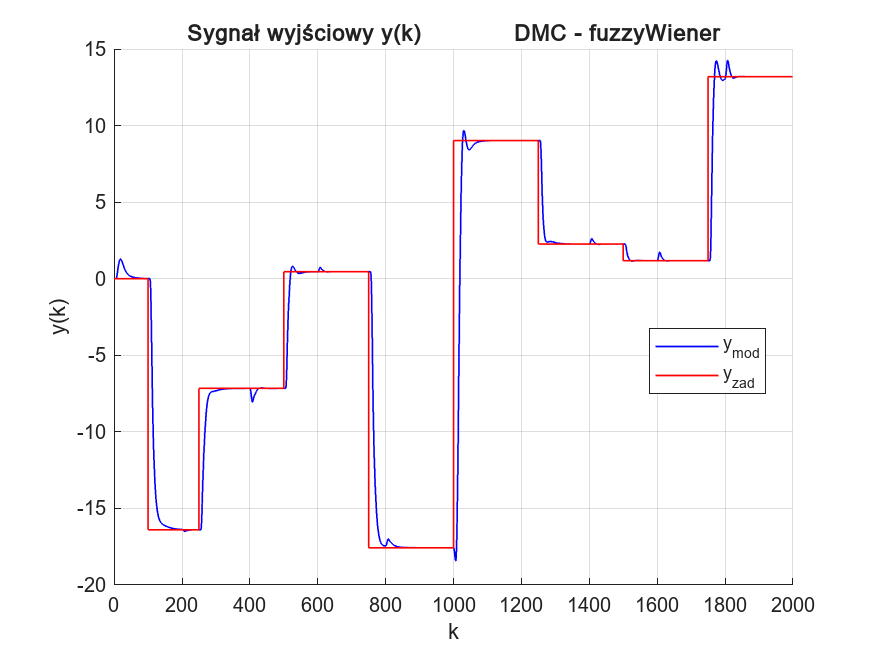
\includegraphics[width=\linewidth]{pictures/y_fuzzyWiener}
\caption{Wiener - sygnał wyjściowy $y(k)$.}
\end{subfigure}
\hfill
\begin{subfigure}[b]{0.49\paperwidth}
\centering
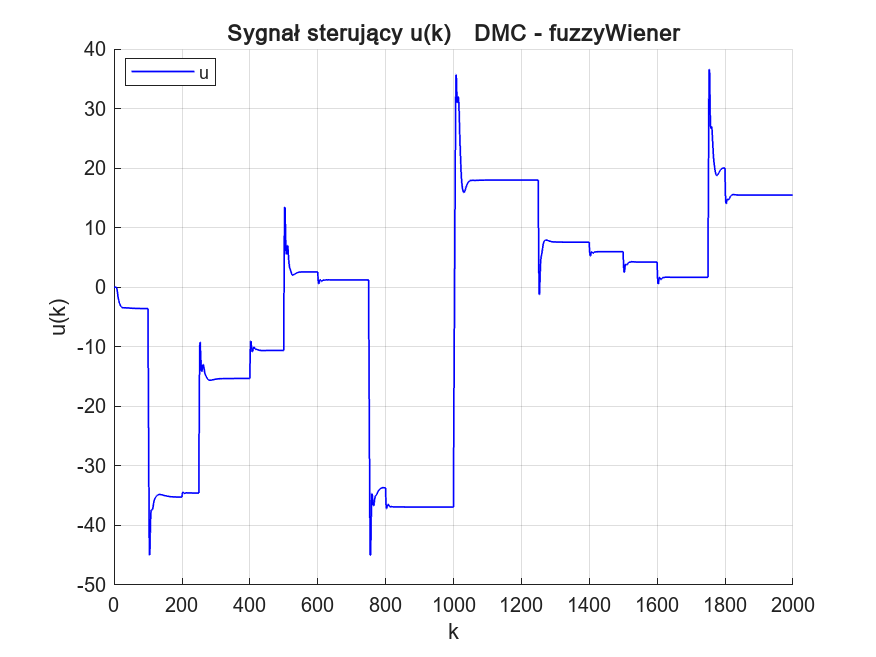
\includegraphics[width=\linewidth]{pictures/u_fuzzyWiener}
\caption{Wiener - sygnał sterujący $u(k)$.}
\end{subfigure}

\caption{Regulator FDMC.}
\end{figure}

\restoregeometry 
\newpage

Wskaźnik jakości użyty do określenia jakości wyznaczonego sterowania był postaci:

\begin{equation}
J = \sum_{i=1}^N (y_{zad}(i) - y(i))^2 + \lambda \sum_{i=1}^N \Delta u(i)^2
\end{equation}

Zatem uwzględniłem zarówno uchyby regulacji, jak i zmiany sygnału sterującego. Wartości wskaźnika zamieściłem w tabeli poniżej.

\begin{table}[h!]
\centering
\begin{tabular}{|>{\raggedright\arraybackslash}p{4cm}|>{\centering\arraybackslash}p{4cm}|>{\centering\arraybackslash}p{4cm}|} 
\hline
Regulator & Hammerstein & Wiener \\ \hline
DMC - analityczny & $25214.753$ & $25130.851$ \\ \hline 
DMC - numeryczny & $25214.753$ & $25130.851$ \\ \hline 
DMC - SL & $24605.791$ & $24568.536 $ \\ \hline 
DMC - NPL & $24490.601$ & $24464.042$ \\ \hline 
FDMC & $23555.099$ & $23636.443$ \\ \hline 
\end{tabular}
\caption{Porównanie regulatorów.}
\end{table}

Zgodnie z wiedzą teoretyczną, bardziej złożone regulatory pozwoliły z większą dokładnością odwzorować sygnał zadany. \textbf{Zastanawiam się nad faktem, że regulatory analityczne i numeryczne dały dokładnie te same wyniki oraz przebiegi sygnałów wyjściowego i sterującego.}